\chapter[Gestione professori]{Professori: gestione spazio personale}


\begin{figure}[H]
 \centering
 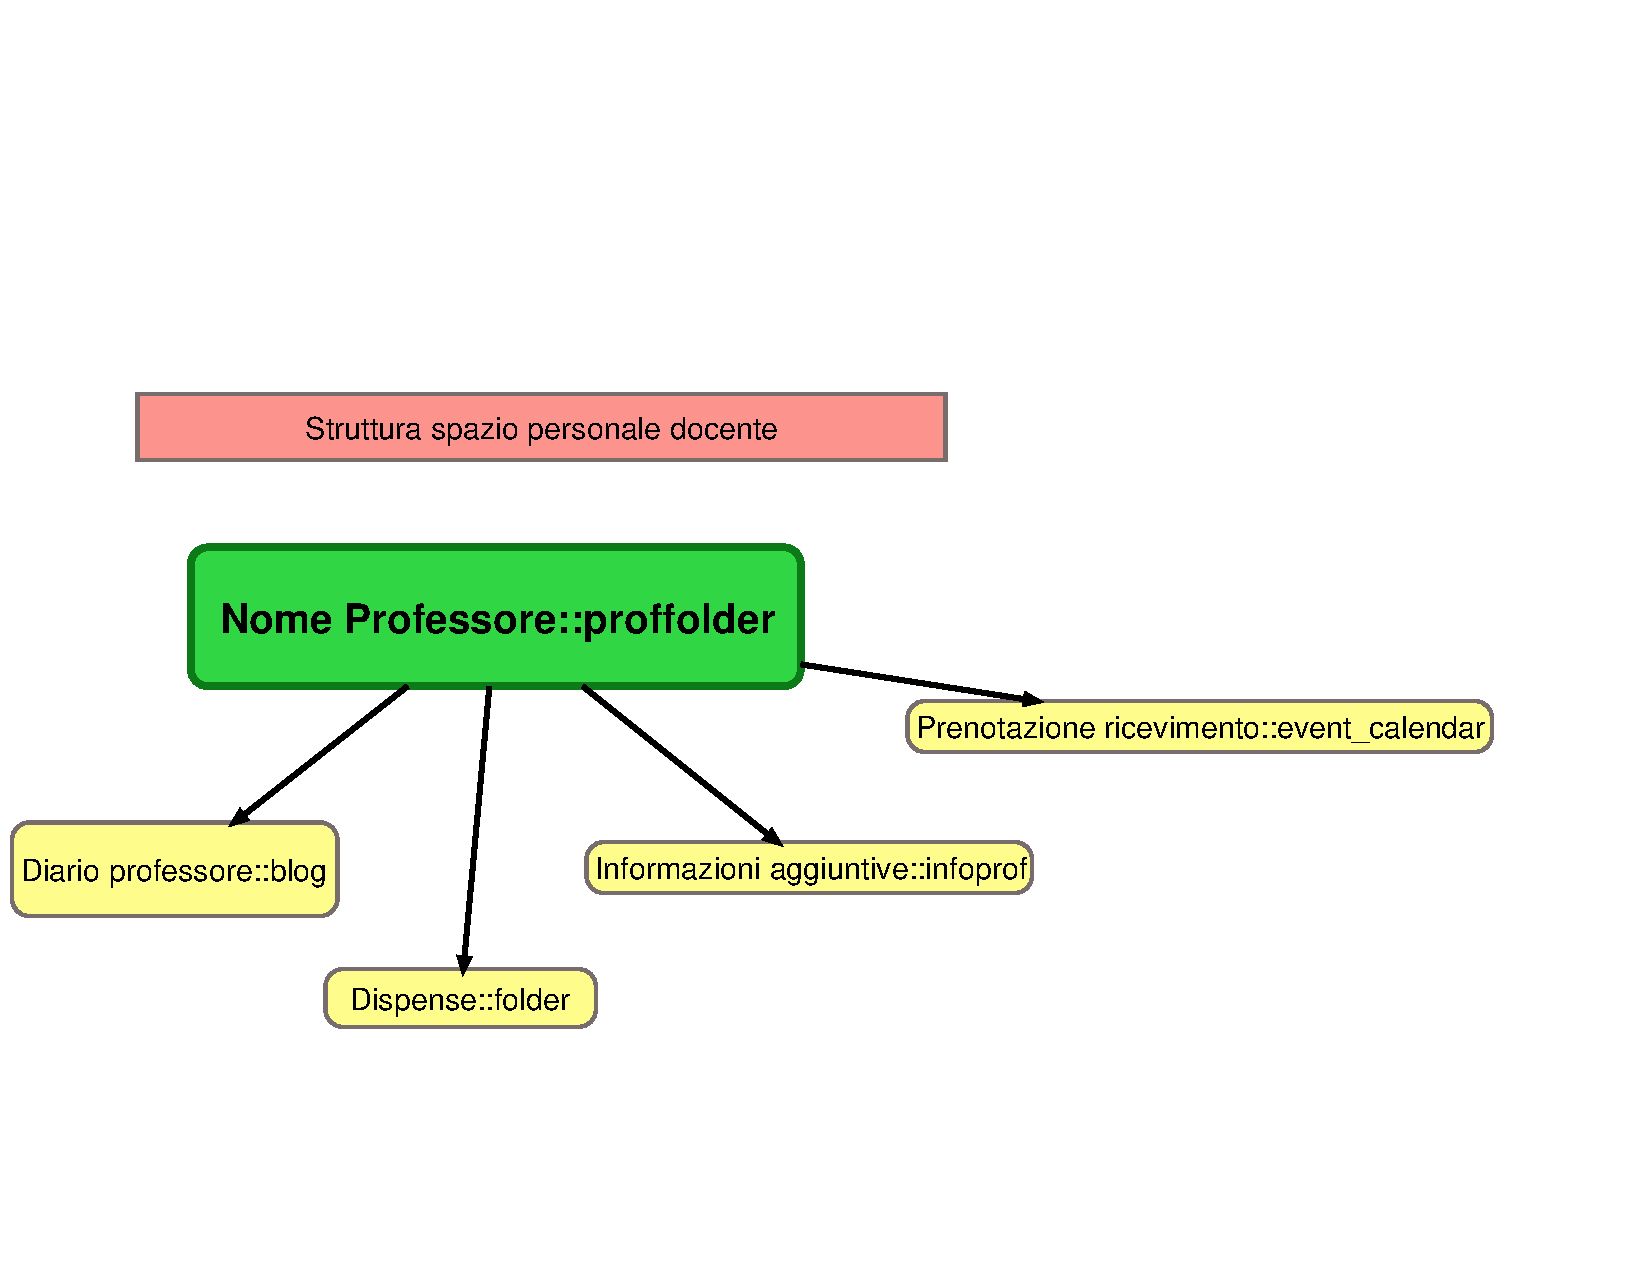
\includegraphics[width=\textwidth]{./immagini/prof_guide/struttura_spazio_docente.pdf}
 % struttura_spazio_docente.pdf: 792x612 pixel, 72dpi, 27.94x21.59 cm, bb=
 \caption{Struttura dello spazio docente creata durante la fase di registrazione}
 \label{fig:proffolder_structture}
\end{figure}



Ogni docente ha a disposizione uno  (o più) spazi personali all'interno dei quali può caricare contenuti utili all'attività didattica. La Collocazione di ogni spazio personale è:
\begin{verbatim}
 \Home\<Nome scuola>\Docenti\<Nome docente>
\end{verbatim}
se un insegnante lavora in più scuole gestite dall'istituto in ognuna di queste avrà a disposizione uno spazio personale diversificato in cui inserire i suoi contenuti.

\begin{figure}[H]
 \centering
 \includegraphics[width=\textwidth]{./immagini/prof_guide/user_links.png}
 % user_links.png: 578x38 pixel, 72dpi, 20.39x1.34 cm, bb=
 \caption{Link accessibili all'utente registrato}
 \label{fig:user_links}
\end{figure}

Oltre allo spazio personale ogni insegnate dispone di un profilo personale, non visibile pubblicamente, tramite il quale può gestire le sue relazione con la struttura scolastica (classi di insegnamento, plessi di insegnamento, collocazione geografica della sede di lavoro). Per accedere al profilo personale è sufficiente, una volta effettuato il login, cliccare con il mouse sui link presenti nella parte alta della pagina figura.\ref{fig:user_links}

Verrà quindi visualizzato il profilo personale. In  tal pagina sarà possibile modificare le proprie preferenze operative, cambiare il proprio avatar etc. Nel caso di un insegnate, ovvero di un utente con a disposizione uno spazio personale verranno anche elencati tali spazi figura.\ref{fig:vista_profilo_utente}
\begin{figure}[h]
 \centering
 \includegraphics[width=\textwidth]{./immagini/prof_guide/prof_profile0.png}
 % prof_profile0.png: 1173x590 pixel, 72dpi, 41.38x20.81 cm, bb=
 \caption{Vista generale del profilo utente professore}
 \label{fig:vista_profilo_utente}
\end{figure}

Per modificare il profilo personale è sufficiente cliccare con il mouse sul pulsante \textsl{Modifica}, comparirà la pagina di modifica all'interno della quale andremo ad impostare le preferenze. Figura.\ref{fig:profile_edit1}

\begin{figure}[H]
 \centering
 \includegraphics[width=\textwidth]{./immagini/prof_guide/prof_profil1.png}
 % personal_prof1.png: 1063x421 pixel, 72dpi, 37.50x14.85 cm, bb=
 \caption{Modifica del profilo personale: è possibili modificare i propri dati come nome,cognome, password, indirizzo e-mail}
 \label{fig:profile_edit1}
\end{figure}
È possibile caricare un'immagine che sarà utilizzata nello spazio personale docente e specificare le scuole in cui si insegna. Figura.\ref{fig:profile_edit2}

\begin{figure}[H]
 \centering
 \includegraphics[width=\textwidth]{./immagini/prof_guide/prof_profile_2.png}
 % personal_prof2.png: 1071x111 pixel, 72dpi, 37.78x3.92 cm, bb=
 \caption{È possible caricare una  proprio foto nel profilo utente}
 \label{fig:profile_edit2}
\end{figure}
Quando le classi di insegnamento cambiano è possibile riassociare lo spazio personale insegnante alle nuove classi. Figura.\ref{fig:edit_profile3}

\begin{figure}[H]
 \centering
 \includegraphics[width=\textwidth]{./immagini/prof_guide/prof_profile3.png}
 % prof_profile3.png: 1244x642 pixel, 72dpi, 43.89x22.65 cm, bb=
 \caption{Modifica delle classi di insegnamento}
 \label{fig:edit_profile3}
\end{figure}
\section{Inserimento dati nello spazio personale}

\subsection{Attivazione spazio personale}
Per poter rendere disponibile nella sezione pubblica del sito il proprio spazio personale, dopo l'attivazione il docente deve modificare lo stato dell'oggetto di Classe Prof Folder istanziato durante la creazione dell'account.
Per far questo, dopo aver effettuato il login ed essersi posizionato nella cartella personale:
\begin{verbatim}
 <Scuola>/Docenti/<Nome Docente>
\end{verbatim}

deve cliccare sul tasto:
 \includegraphics[bb=0 0 26 32]{./immagini/edit/tasto_stato.png} 
e nella finestra di dialogo per l'impostazione degli stati selezionare \textsl{Pronto}:
\begin{figure}[H]
 \centering
 \includegraphics[width=\textwidth]{./immagini/prof_guide/stati_docente.png}
 % stati_docente.png: 1245x164 pixel, 72dpi, 43.92x5.79 cm, bb=
 \caption{Impostate lo stato come pronto visualizzare lo spazio personale nella sezione pubblica del sito}
 \label{fig:stati_docente}
\end{figure}





Se l'insegnate ha sufficienti permessi, quando si trova all'interno del suo spazio personale comparirà una barra degli strumenti subito sotto il menu a tendina figura.\ref{fig:toolbar_1}. Tramite questa barra sarà possibile creare dei contenuti all'interno dello spazio personale o modificare quelli già presenti figura.\ref{fig:toolbar_2}.

\begin{figure}[H]
 \centering
 \includegraphics[width=\textwidth]{./immagini/prof_guide/toolbar_1.png}
 % toolbar_1.png: 242x44 pixel, 72dpi, 8.54x1.55 cm, bb=
 \caption{Toolbar per la creazione dei contenuti: scelta della classe}
 \label{fig:toolbar_1}
\end{figure}

\begin{figure}[H]
 \centering
 \includegraphics[width=\textwidth]{./immagini/prof_guide/toolbar2.png}
 % toolbar2.png: 236x51 pixel, 72dpi, 8.33x1.80 cm, bb=
 \caption{Azioni disponibili all'utente}
 \label{fig:toolbar_2}
\end{figure}
Nello spazio personale è possibile inserire dei recapiti diversi da quelli inseriti nel profilo utente. Nella schermata principale dello spazio personale sono immediatamente visibili le classi di insegnamento del docente. Figura.\ref{fig:prof_personal22}

\begin{figure}[H]
 \centering
 \includegraphics[width=\textwidth]{./immagini/prof_guide/personal_prof1.png}
 % personal_prof1.png: 1063x421 pixel, 72dpi, 37.50x14.85 cm, bb=
 \caption{Layout profilo personale professore}
 \label{fig:personal_prof1}
\end{figure}
All'interno di ogni spazio personale il docente dovrebbe creare un oggetto di tipo infoProf all'interno del quale inserire:
\begin{itemize}
\item Le materie insegnate nella scuola cui appartiene il presente spazio personale
\item Gli orari di ricevimento nella scuola cui appartiene il presente spazio personale
\item L'orario delle lezioni nella scuola cui appartiene il presente spazio personale
\end{itemize}

in questo modo gli utenti del sito potranno filtrare gli insegnanti in funzione di vari parametri

\begin{figure}[H]
 \centering
 \includegraphics[width=\textwidth]{./immagini/prof_guide/infoprof.png}
 % infoprof.png: 425x41 pixel, 72dpi, 14.99x1.45 cm, bb=
 \caption{Ogni insegnante dovrebbe creare un oggetto di tipo infoProf in cui caricare le matarie di insegmanto, gli orari di ricevimento etc. per ogni scuola}
 \label{fig:infoprof_crea}
\end{figure}
\begin{figure}[H]
 \centering
 \includegraphics[width=\textwidth]{./immagini/prof_guide/infoprof1.png}
 % infoprof1.png: 1245x620 pixel, 72dpi, 43.92x21.87 cm, bb=
 \caption{Durante la creazione o la modifica di un oggetto infoProf è possibile inserire le materie di insegmento, gli orari di ricevimento e l'orario delle lezioni.}
 \label{fig:infoprof_edit1}
\end{figure}


\begin{figure}[H]
 \centering
 \includegraphics[width=\textwidth]{./immagini/prof_guide/personal_prof2.png}
 % personal_prof2.png: 1071x111 pixel, 72dpi, 37.78x3.92 cm, bb=
 \caption{Classi associate a questo profilo docente}
 \label{fig:prof_personal22}
\end{figure}
\begin{figure}[H]
 \centering
 \includegraphics[width=0.8\textwidth]{./immagini/prof_guide/personal_prof3.png}
 % personal_prof3.png: 143x180 pixel, 72dpi, 5.04x6.35 cm, bb=
 \caption{Contenuti caricati dal docente}
 \label{fig:prof_personal3}
\end{figure}

\section{Feedback Form}

Ogni docente può creare nel suo spazio personale un oggetto di classe Formulario feedback per permettere agli utenti del sito di comunicare con lui. Per la creazione di un oggetto di tal classe procediamo nella solita maniera: dalla barra degli strumenti selezioniamo la voce \textsl{Formulario feedback} e creiamo l'oggetto:
\begin{figure}[H]
 \centering
 \includegraphics[width=\textwidth]{./immagini/prof_guide/feedback_form.png}
 % feedback_form.png: 1242x679 pixel, 72dpi, 43.81x23.95 cm, bb=
 \caption{Formulario per ricevere informazioni dagli utenti}
 \label{fig:feedback_form}
\end{figure}
\section{Classi}

I docenti possono gestire le classi di insegnamento, inserendo contenuti ed informazioni. Il procedimento per la gestione/creazione delle pagine è analogo a quello esposto in questo capitolo. Il docente dovrà avere unicamente l'accortezza di posizionarsi all'interno della classa prescelta. L'indirizzo standard delle classi è:
\begin{verbatim}
 Home\<Scuola>\Classi\<Classe>
\end{verbatim}
Lo stato iniziale delle classi è \textsl{in preparazione} il docente dovrà quindi impostare lo stato a \textsl{pronto} quando riterrà opportuno rendere pubblici i contenuti.